\chapter{Závěr}
V této kapitole budou shrnut současný stav aplikace,
  nápadu na její vylepšení,
  porovnání s podobnými aplikacemi a
  na úplný závěr bude zmíněny problémy,
  na které jsem narazil při vývoji nástroje MT-ComparEval.

\section{Současný stav aplikace}
Nástroj MT-ComparEval je v současné době plně funkční.
Umožňuje spravovat experimenty a jejich tasky.
Tasky je možné porovnávat na základě různých kriterií -
  hodnot metrik strojového překladu,
  porovnání jednotlivých vět
  či přehledu nejvíce zlepšujících a zhoršujících n-gramů.
Při porovnání překladů jedné věty je možné si nechat zvýraznit
  potvrzené n-gramy, zlepšující n-gramy, zhoršující n-gramy, diff mezi překlady
  či jeden z nejvíce zlepšujících nebo zhoršujících n-gramů.

To vše by mělo sloužit k usnadnění vyhodnocování a porovnávání překladů,
  které musí vývojář strojových překladačů pravidelně provádět.

\section{Nápady na vylepšení}
I přes to, že nástroj MT-ComparEval umožňuje porovnávat dvě různé verze překladů,
  existuje mnoho způsobů,
  jak by tento nástroj šlo vylepšit.
Některé z těchto nápadů budou představeny v následující části.

\subsection{Podpora více referencí}
Při vyhodnocování strojových překladů a počítání metrik používá nástroj MT-ComparEval pouze porovnání s jednou referencí.
Avšak většina vět může být přeložena různými způsoby,
  které nemusí odpovídat zvolené referenci.
Aby bylo možné lépe ohodnotit překlady,
  mohly by být překlady porovnávány s několika různými referencemi,
  z nichž by se vybrala ta,
  pro kterou by daný překlad dosáhl nejlepšího skóre.
Kvůli tomu by bylo třeba přidat podporu více referencí v experimentu.

\subsection{Více metrik}
I když metrika BLEU silně odpovídá lidskému hodnocení překladů,
  nemusí být považována za nejvhodnější pro vyhodnocování překladů.
Některé strojové překladače jsou speciálně optimalizovány na metriku BLEU,
  což ve výsledku nemusí dávat zcela vhodné překlady.
Proto je vhodné,
  aby byly strojové překladače vyhodnocovány na základě několika metrik.
Mezi metriky,
  které by bylo vhodné do nástroje MT-ComparEval doprogramovat,
  patří např. NIST, METEOR, PORT,~\dots

\subsection{Zobrazení alignmentu}
Při porovnávání dvou překladů jedné věty,
  by uživatelům mohla přijít vhod funkce pro zvýraznění slov,
  které odpovídají danému slovu v referenci či dalším strojovém překladu.
Tomu se říká \textbf{alignment}.
Díky této funkci by pak uživatelé mohli snadněji analyzovat chovaní strojových překladačů.

Na Obrázku \ref{img:alignment} je možné vidět, jak zvýrazňuje aligment překladač Google Translate.
\begin{figure}
	\center
	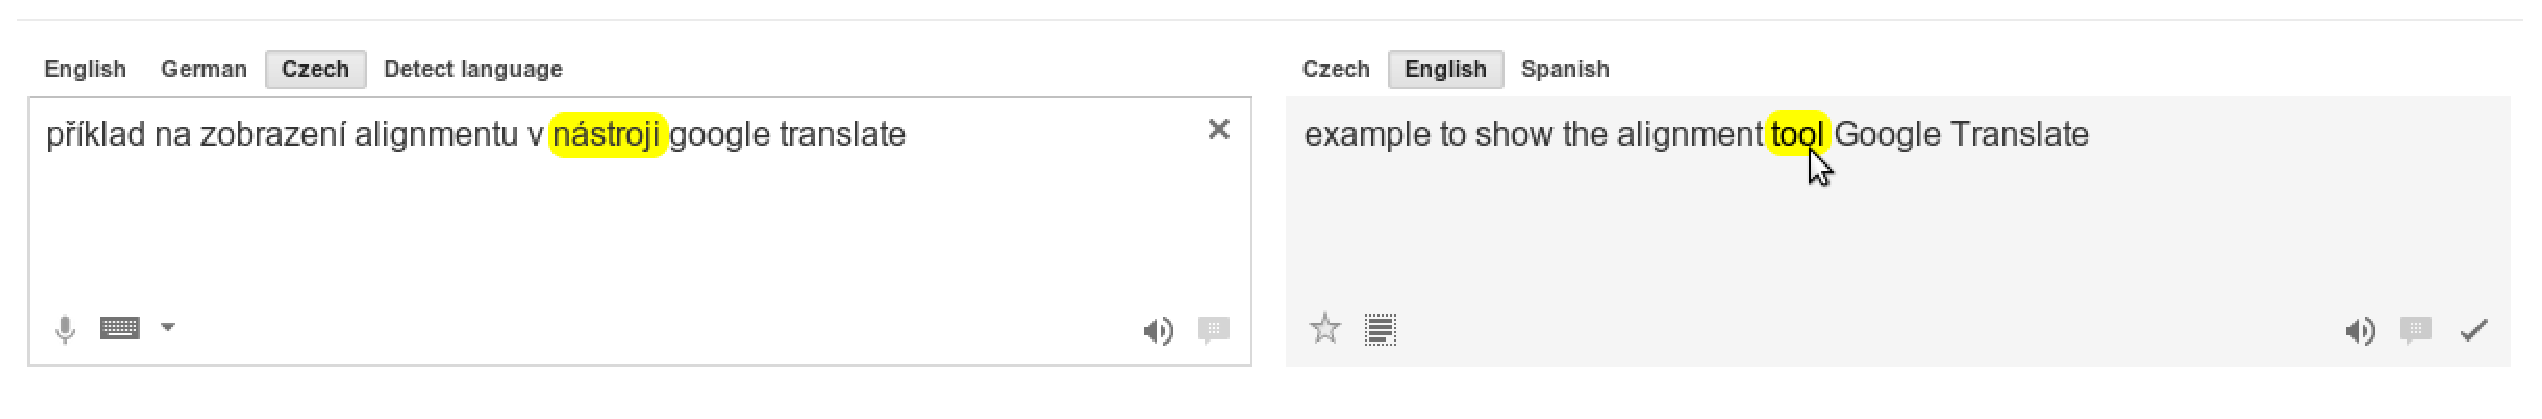
\includegraphics[width=0.9\textwidth]{img/alignment.eps}
	\caption{Ukázka zobrazení aligmentu v překladači Google Translate}
	\label{img:alignment}
\end{figure}

\section{Podobné aplikace}
Vývoj nástroje MT-ComparEval byl v určitých oblastech inspirován nástroji,
  které už mohou vývojáři běžně využívat při své práci.
Z těchto nástrojů byly vybrány nejdůležitější vlastnosti,
  které byly později zkombinovány do jednoho funkčního celku.
V následující části budou tyto nástroje podrobněji představeny.

\subsection{mteval-11b.pl}
Je skript napsaný v jazyce Perl,
  který umožňuje počítat metriky BLEU a NIST.
Tento skript je celosvětově používaný,
  a proto byl použit pro kontrolu,
  že metriku BLEU v MT-ComparEval počítáme správně.

V současné době už existuje verze mteval-13a.pl,
  v které mimojiné přibyla možnost počítat metriky pro jednotlivé segmenty v překladu.

\subsection{iBLEU}
Nástroj iBLEU umožňuje vyhodnocovat a porovnávat strojové překlady.
Pokud uživatel nemá žadný jiný strojový překlad,
  s kterým by chtěl svůj překlad porovnat,
  může si větu nechat přeložit překladačem Google Translate\footnote{
    Bohužel Google Translate nenabízí bezplatné api.
  } nebo Bing Translator\footnote{
    Bing Translator nabízí bezplatné api do limitu 2 miliónů přeložených znaků za den.
  }
  a porovnat svůj překlad s překladem z tohoto nástroje.

Pomocí tohoto nástroje můžeme počítat BLEU pro celé dokumenty nebo i jednotlivé segmenty
  a podle jejich výsledku si je můžeme později prohléhnout.

Pokud uživatel porovnává svůj strojový překlad pouze s referenčním překladem,
  je zvýrazněn jejich diff.
V případě, že uživatel porovnává dva strojové překlady,
  je zobrazen diff těchto překladů.

Tento nástroj je možné používat lokálně jako webovou aplikaci bez použití webového serveru,
  protože je celý napsán v HTML 5, CSS a javascriptu.
Stejně jako MT-ComparEval i iBLEU používá pro počítání BLEU jako referenční implementaci mteval-13a.pl.

Na Obrázku \ref{img:ibleu} je možné vidět porování dvou překladů v nástroji iBLEU.
\begin{figure}
  \center
  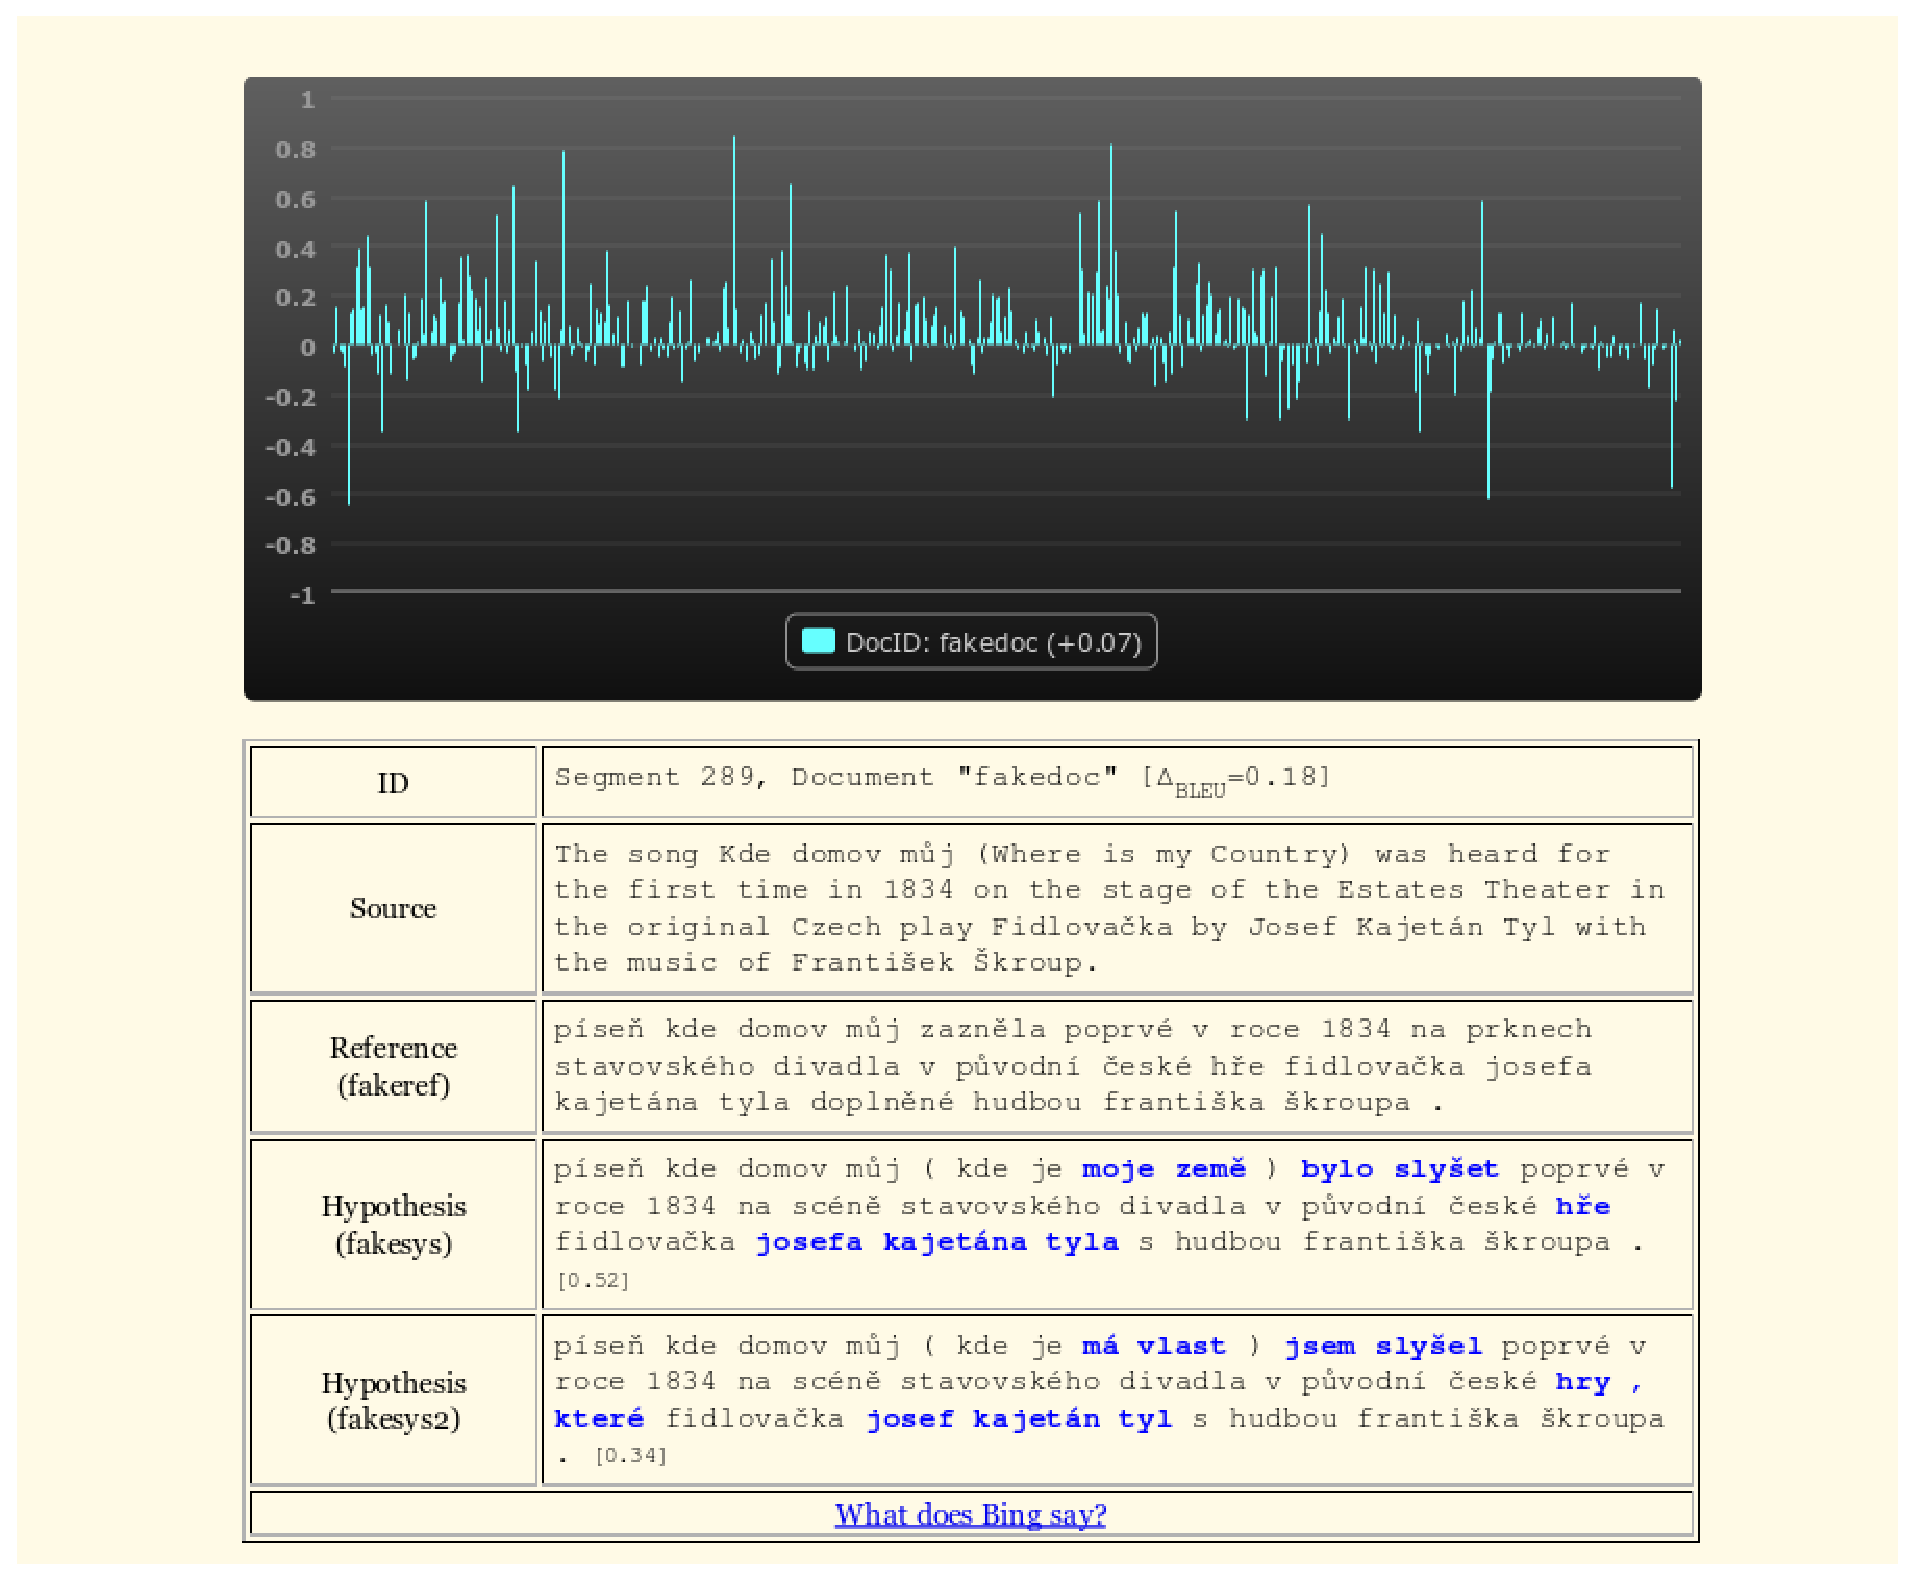
\includegraphics[width=0.9\textwidth]{img/ibleu.eps}
  \caption{Porovnání dvou překladů v nástroji iBLEU}
  \label{img:ibleu}
\end{figure}


\subsection{EMS - An Experimental Management System}
Nástroj EMS,
  který je součástí strojového překladače Moses,
  obsahuje webovou aplikaci,
  díky níž je možné porovnávat překlady.
V porovnávaných větách barevně zvýrazňuje slova,
  na základě délky nejdelšího n-gramu,
  do kterého zvýrazňované slovo patří.
Obrázek \ref{img:ems-sentence} ukazuje takto zvýrazněnou větu.
Pro n-gramy také počítá precision a recall.

\begin{figure}
  \caption{Zvýrazněné n-gramy podle délky v nástroji EMS}
  \label{img:ems-sentence}
\end{figure}

Ve webovém prostředí je též možné vyhledávat věty,
  ve kterých byl použit n-gram.
Jednotlivá užití n-gramů jsou pak rozřazena do skupin podle správnosti překladu.
Na Obrázku \ref{img:ems-word} je možné vidět seznam vět,
  ve kterých bylo použito slovo ??.

\begin{figure}
  \caption{Výpis vět, ve kterých se vyskytuje slovo ??, v nástroji EMS}
  \label{img:ems-word}
\end{figure}

Další věcí, kterou můžeme použít při porovnávání dvou překladů,
  jsou grafy správně přeložených vs. špatně přeložených slov.
Takové grafy je možné vidět na Obrázku \ref{img:ems-charts}.

\begin{figure}
  \caption{Grafy správně přeložených vs. špatně přeložených slov v nástroji EMS}
  \label{img:ems-charts}
\end{figure}

Webové prostředí nástroje EMS nabízí i další možnosti porovnání překladů,
  o kterých je možné se více dozvědět v dokumentaci tohoto nástroje.

\section{Problémy při řešení}
Při vývoji nástroje MT-ComparEval jsem narazil na mnoho problémů.
Ať už se jednalo o volbu jazyka, frameworku či databáze.

Z počátku byl nástroj MT-ComparEval vyvíjen v jazyce Perl,
  ale po několika neúspěšných pokusech byl nahrazen za jazyk PHP,
  ve kterém jsem více zběhlý.
Jelikož většina nástrojů pro strojový překlad je vyvíjena v jazyce Perl,
  nelze mu připisovat žádné mínusové body.
Chyba byla v tomto případě na mé straně.

Aby bylo možné snadno nainstalovat nástroj MT-ComparEval na vývojářově počítači,
  byla jako databáze zvolena databáze SQLite 3.
Ta vyhovuje většině požadavků.
Bohužel jsem strávil hodně času s odhalováním chyb,
  způsobených tím,
  že SQLite 3 zamyká zvláštním způsobem datový soubor,
  a proto není možné používat databázi v různých procesech.
Při normálním použití na webu se s touto chybou nepotkáme,
  protože procesy databázi používají pouze během zpracování HTTP požadavku.
Avšak při použití dlouho trvajících procesů pro import experimentů a tasků
  vždy docházelo ke kolizím při přístupu k databázi,
  které vyústili v pád importu.
Proto musel být návrh importu zcela přepracován a nyní by měl fungovat podle představ.


V duchu TDD\footnote{Test-Driven-Development}
  jsem se snažil před vlastní implementací napsat testy pomocí nástroje Behat.\footnote{http://www.behat.org}
Ten slouží k BDD\footnote{Behaviour-Driven-Development}.
Pro všechny kroky importů byly napsáný specifikace chování, které byly nástrojem Behat otestovány.
Ovšem později se ukázalo, že tento přístup k testování nebyl úplně vhodný, a testy pomocí tohoto nástroje jsem přestal psát.
Vše bylo způsobeno tím, že byla porušena pyramida testů\footnote{http://martinfowler.com/bliki/TestPyramid.html},
  jelikož všechny testy odpovídali funkčním testům.
Lepší přístup by byl vytvořit pro všechny funkční požadavky unit testy,
  jejichž spuštění by trvalo kratší dobu.
